\xiti
\begin{xiaotis}
\begin{enhancedline}

\xiaoti{已知圆的半径等于 5 cm,圆心到直线 $l$ 的距离是:(1)3 cm; (2)5cm;(3) 7 cm。
    直线 $l$ 和圆有几个交点?为什么?
}

\xiaoti{如图,可以利用刻度尺和三角板测量圆形工件的直径。说明测量的道理。}

\begin{figure}[htbp]
    \centering
    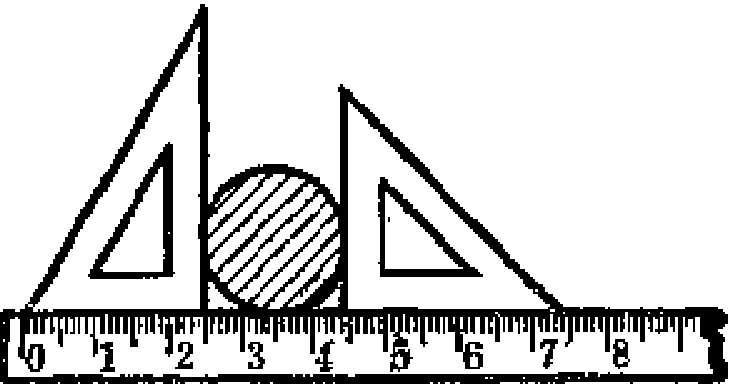
\includegraphics[width=8cm]{../pic/czjh2-ch7-xiti25-02.png}
    \caption*{(第 2 题)}
\end{figure}

\xiaoti{已知:如图, $\triangle ABC$ 内接于 $\yuan\,O$, $\angle CAE = \angle B$。如果
    (1) $AB$ 是直径; (2)$AB$ 为非直径的弦,
    求证: $AE$ 与 $\yuan\,O$ 相切于点 $A$。
}

\begin{figure}[htbp]
    \centering
    \begin{minipage}[b]{9cm}
        \centering
        \begin{minipage}[b]{4.4cm}
            \begin{tikzpicture}
    \tkzDefPoints{0/0/O}
    \tkzDefPoint(180:1.5){A}
    \tkzDefPoint(0:1.5){B}
    \tkzDefPoint(300:1.5){C}
    \tkzDefLine[perpendicular=through A,normed](O,A)  \tkzGetPoint{e}
    \tkzDefPointOnLine[pos=1.5](A,e)  \tkzGetPoint{E}

    \tkzDrawCircle[thick](O,A)
    \tkzDrawPoint(O)
    \tkzDrawPolygon(A,B,C)
    \tkzDrawLine[add=0 and 1](E,A)
    \tkzMarkAngle[size=.5](A,B,C)
    \tkzMarkAngle[size=.5](E,A,C)
    \tkzLabelPoints[below](O)
    \tkzLabelPoints[left](A)
    \tkzLabelPoints[right](B)
    \tkzLabelPoints[below](C)
    \tkzLabelPoints[left](E)
\end{tikzpicture}


        \end{minipage}
        \begin{minipage}[b]{4.4cm}
            \begin{tikzpicture}
    \tkzDefPoints{0/0/O}
    \tkzDefPoint(180:1.5){A}
    \tkzDefPoint(20:1.5){B}
    \tkzDefPoint(300:1.5){C}
    \tkzDefLine[perpendicular=through A,normed](O,A)  \tkzGetPoint{e}
    \tkzDefPointOnLine[pos=1.5](A,e)  \tkzGetPoint{E}

    \tkzDrawCircle[thick](O,A)
    \tkzDrawPoint(O)
    \tkzDrawPolygon(A,B,C)
    \tkzDrawLine[add=0 and 1](E,A)
    \tkzMarkAngle[size=.5](A,B,C)
    \tkzMarkAngle[size=.5](E,A,C)
    \tkzLabelPoints[below](O)
    \tkzLabelPoints[left](A)
    \tkzLabelPoints[right](B)
    \tkzLabelPoints[below](C)
    \tkzLabelPoints[left](E)
\end{tikzpicture}


        \end{minipage}
        \caption*{(第 3 题)}
    \end{minipage}
    \qquad
    \begin{minipage}[b]{5.6cm}
        \centering
        \begin{tikzpicture}
    \pgfmathsetmacro{\R}{1.8}
    \pgfmathsetmacro{\r}{1.4}

    \tkzDefPoints{0/0/O_2}
    \tkzDefPoint(180:\R){O_1}
    \tkzDefPoint(0:\R){C}
    \tkzInterCC[R](O_1,\r)(O_2,\R)  \tkzGetPoints{A}{B}

    \tkzDrawCircle[thick](O_1,A)
    \tkzDrawCircle[thick](O_2,A)
    \tkzDrawPoints(O_1, O_2)
    \tkzDrawSegments(O_1,C  A,C)

    \tkzLabelPoints[left](O_1)
    \tkzLabelPoints[below](O_2)
    \tkzLabelPoints[above=.2em](A)
    \tkzLabelPoints[below=.2em](B)
    \tkzLabelPoints[right](C)
\end{tikzpicture}


        \caption*{(第 4 题)}
    \end{minipage}
\end{figure}

\xiaoti{$\yuan\,O_2$ 经过 $\yuan\,O_1$ 的圆心, 与 $\yuan\,O_1$ 相交于 $A$、$B$ 两点。
    直线 $O_1O_2$ 交 $\yuan\,O_2$ 于点 $C$。
    求证: $AC$ 是 $\yuan\,O_1$ 的切线。
}

\xiaoti{两个同心圆中,大圆的弦 $AB$ 和 $AC$ 分别和小圆相切于点 $D$ 和 $E$。
    求证: $DE \pxqdy \exdfrac{1}{2} BC$。
}

\xiaoti{$MN$ 是 $\yuan\,O$ 的切线, $AB$ 是 $\yuan\,O$ 的直径。
    求证: 点 $A$ 、$B$ 与 $MN$ 的距离的和等于 $\yuan\,O$ 的直径。
}

\xiaoti{设 $AB$ 为 $\yuan\,O$ 的直径, $C$ 是 $\yuan\,O$ 上一点,
    $AD$ 和 $\yuan\,O$ 在点 $C$ 的切线相垂直,垂足为 $D$。
    求证: $AC$ 平分 $\angle DAB$。
}

\xiaoti{求证:以等腰三角形底边的中点为圆心,并且和一腰相切的圆,也和另一腰相切。}

\xiaoti{}%
\begin{xiaoxiaotis}%
    \xxt[\xxtsep]{作一个半径为 3 cm的圆,使它与已知直线 $l$ 相切于 $l$ 上一点 $A$;}

    \xxt{以直线 $l$ 外一点 $A$ 为圆心,作圆与直线 $l$ 相切。}

\end{xiaoxiaotis}

\xiaoti{已知:等腰梯形各边都与 $\yuan\,O$ 相切, $\yuan\,O$ 的直径为 6 cm,
    等腰梯形的腰等于 8 cm。 求梯形的面积。
}

\xiaoti{$PA$、$PB$ 是 $\yuan\,O$ 的切线, $A$、$B$ 是切点, 延长半径 $OB$ 到 $C$,
    使 $BC = OB$。 求证: $\angle APC = 3 \angle BPC$。
}

\xiaoti{$AB$、$CD$ 是 $\yuan\,O$ 的切线, $AB \pingxing CD$;
    $EF$ 也是 $\yuan\,O$ 的切线,它和 $AB$、$CD$ 分别相交于点 $E$ 和 $F$。
    求证: $\angle EOF = 90^\circ$。
}

\xiaoti{$PA$、$PB$ 为 $\yuan\,O$ 的切线, $AC$ 为经过切点 $A$ 的直径。
    求证: 切点 $B$ 和点 $C$ 的连线平行于 $PO$。
}

\xiaoti{过 $\yuan\,O$ 外的一点 $P$ 的直线 $PA$ 和 $PB$ 与 $\yuan\,O$ 相切于点 $A$ 和 $B$。
    $D$ 是 $\yuanhu{AB}$ 上任意一点, 过点 $D$ 的切线与 $PA$ 和 $PB$ 分别相交于点 $E$ 和 $F$。
    已知 $\angle P = \alpha$, 用 $\alpha$ 表示 $\angle EOF$。
}


\xiaoti{求证:}
\begin{xiaoxiaotis}

    \xxt{等边三角形的内心也是它的外心;}

    \xxt{等边三角形的外接圆半径 $R$ 是内切圆半径 $r$ 的 2 倍。}

\end{xiaoxiaotis}

\xiaoti{$\triangle ABC$ 中,内切圆 $I$ 和边 $BC$、$CA$、$AB$ 分别相切于点 $D$、$E$、$F$。
    求证: $\angle FDE = 90^\circ - \exdfrac{1}{2} \angle A$。
}

\xiaoti{$\triangle ABC$ 中, $E$ 是内心, $\angle A$ 的平分线和 $\triangle ABC$
    的外接圆相交于点 D。 求证: $DE = DB = DC$。
}

\xiaoti{圆外切四边形的周长为 48 厘米, 相邻的三条边的比为 $5:4:7$, 求四边形各边的长。}

\xiaoti{$ABCDEF$ 是 $\yuan\,O$ 的外切六边形。求证:
    $$ AB + CD + EF = BC + DE + FA \juhao $$
}

\xiaoti{已知: $\triangle ABC$ 的 $\angle A$ 的平分线和外接圆 $O$ 相交于点 $D$,
    $BE$ 是 $\yuan\,O$ 的切线。 求证: 点 $D$ 到 $BC$ 和到 $BE$ 的距离相等。
}

\xiaoti{$\yuan\,O$ 的弦 $AB$ 的延长线和切线 $EP$ 相交于点 $P$, $E$ 为切点。
    $\angle APE$ 的平分线和 $AE$、$BE$ 分別相交于点 $C$、$D$。
    求证: $\triangle CDE$ 是等腰三角形。
}

\xiaoti{已知: $PA$、$PB$ 与 $\yuan\,O$ 相切于点 $A$、$B$, $AC$ 是 $\yuan\,O$ 的直径。
    求证: $\angle APB = 2 \angle BAC$。
}

\begin{figure}[htbp]
    \centering
    \begin{minipage}[b]{7cm}
        \centering
        \begin{tikzpicture}
    \tkzDefPoints{0/0/O, 3.5/0.5/P}
    \tkzDefPoint(0:1.5){T}

    \tkzDefMidPoint(O,P)  \tkzGetPoint{Q}
    \tkzInterCC(O,T)(Q,P)  \tkzGetPoints{A}{B}
    \tkzDefPointOnLine[pos=2](A,O)  \tkzGetPoint{C}

    \tkzDrawCircle[thick](O,A)
    \tkzDrawPoint(O)
    \tkzDrawSegments(A,C  A,B  P,A  P,B)
    \tkzLabelPoints[left](O)
    \tkzLabelPoints[right](P)
    \tkzLabelPoints[above](A)
    \tkzLabelPoints[below](B)
    \tkzLabelPoints[below](C)
\end{tikzpicture}


        \caption*{(第 22 题)}
    \end{minipage}
    \qquad
    \begin{minipage}[b]{7cm}
        \centering
        \begin{tikzpicture}
    \pgfmathsetmacro{\R}{1.8}
    \pgfmathsetmacro{\r}{1.3}

    \tkzDefPoints{0/0/O}
    \tkzDefPoint(100:\R){A}
    \tkzDefPoint(20:\R){B}
    \tkzDefPoint(210:\r){Y}
    \tkzDefPoint(250:\r){Q}
    \tkzInterLC[common=Y](A,Y)(O,Y)  \tkzGetFirstPoint{X}
    \tkzInterLC[common=Q](B,Q)(O,Y)  \tkzGetFirstPoint{P}

    \tkzDrawCircle[thick](O,A)
    \tkzDrawCircle[thick](O,Y)
    \tkzDrawPoint(O)
    \tkzDrawSegments(A,Y  B,Q)

    \tkzLabelPoints[right](O)
    \tkzLabelPoints[above](A)
    \tkzLabelPoints[right](B)
    \tkzLabelPoints[right, yshift=-.3em](P)
    \tkzLabelPoints[below](Q)
    \tkzLabelPoints[above, xshift=-.2em](X)
    \tkzLabelPoints[below, xshift=-.3em](Y)
\end{tikzpicture}


        \caption*{(第 24 题)}
    \end{minipage}
\end{figure}

\xiaoti{圆内相交两弦中,一弦被交点所内分成的两条线段的长为 4 厘米、7 厘米,
    另一弦全长为 11.5 厘米。 求这弦被分成的两条线段的长。
}

\xiaoti{两个同心圆中, $A$、$B$ 为大圆上的任意两点, 过 $A$、$B$ 作小圆的的割线
    $AXY$ 和 $BPQ$。求证: $AX \cdot AY = BP \cdot BQ$。
}

\xiaoti{作一个正方形,使它的面积等于已知矩形的面积。}

\xiaoti{设 $C$ 为线段 $AB$ 的中点, $BCDE$ 是以 $BC$ 为边的正方形。
    以 $B$ 为圆心, $BD$ 为半径的圆与 $AB$ 及其延长线相交于点 $H$ 及 $K$。求证:
}
\begin{xiaoxiaotis}

    \xxt{$HC \cdot CK = AC^2$;}

    \xxt{$AH \cdot AK = 2 AC^2$。}

\end{xiaoxiaotis}

\end{enhancedline}
\end{xiaotis}

